\useunder{\uline}{\ul}{}
\chapter{Team 5 Agent Design}\label{team_5_agent_design}
\section{Introduction}
\subsection{Leadership Personality}
\noindent When voted leader with fight power our agent practices utilitarianism [1]and promotes actions that maximizes utility and wellbeing of all agents. For Escape the Dark Pitt, the collective aim is to defeat monsters and clear all levels with remaining population above 60 percent. Hence, we can derive utility being inversely related to damage received by agents and deaths. By prioritizing decisions which will bring upon the greatest utility overall even at his own risk and having a selfless concern for other agents, our agent can also be deemed altruistic. But as completing the game is in our agent’s self-interest, it is not pure altruism.
\medskip
\noindent After each monster is defeated, a loot pool is dropped. We believe the loot pool is similar to a Common Pool Resource. All agents have equal opportunities to request for items, deeming the loot pool non-excludable. After an item has been allocated, it is unavailable to other agents, hence the loot pool is also rivalrous in consumption in line with Common Pool Resources. The main difference between the two is the loot pool can be fully depleted each round and fully replenished at the next, while common pool resources generally won’t replenish if it is fully depleted. During loot allocation our agent utilizes theory from equity and desert [1] to aim for fairness and distributive justice by having each agent’s allocation affected by their contribution. Unlike the health points pool, another common pool resource, agents cannot directly contribute to it. We can determine an agent’s contribution by their fight decision as defeating the monster will drop loot, and in turn contribute to the loot pool. Fight decision along with other factors are used to calculate a social network score which will directly impact an agent’s ability to be allocated resource per our algorithm.

\section{Social Network}
If we refer to human interaction in real-life it is also often the case, same person working in development division and at management, division can think and act differently. 
We don’t want to exclude one’s excellence in one filed due to short comes in irrelevant field.
Here we have agent’s algorithm for their fight strategy and algorithm for their leader duties’ functionality potentially been written differently. 
Hence, we establish two different trusts, which can decouple an agent’s strategy quality and leadership goodness, 
This does not mean the trusts are completely independent, 
There are still common factors for both of the trusts.
The irrelevant features are excluded from one to another.¬

Agent uses this these trusts to summaries features from left-hand side and contribute to the decision making of right-hand side. 

Due to the limited size of the game and size of the features, it is sensible to summaries this 2-d personality based on two trust scores

The boundaries for the trust scores both at 0.2 and 0.8 and initial scores at 0.5, all of the agent will be a True Neutral agent at the beginning, and will be the majority for the most of the game time. When developing the logic, True Neutral agents are included in all of the interactions, although priority will be given to some other personalities, but 1), the prioritised agents are small amount due to high standard therefore to make sure there is still the majority of the resource that is left with the bigger amount of agents 2), The accumulated trust addition in a level is less than 0.2 for each of the scores, therefore it will take at least 2 levels for an agent to gain a personality with priority, which ensures enough interaction has happened or enough information is gained for the agent that wen can make a new judgment to its personality. When updating the trust, if there is trust score exceed the region of 0-1, max-min scale is applied to all agent. Under this circumstance, there will be at least one min scored agent and one max scored agent that has two different personalities that is not neutral. 

We don’t want to exclude one’s excellence in one field due to short comes in an irrelevant fields.
Here we have agents’ algorithm for their fight strategy and the algorithm for their leader duties’ functionality potentially written differently. 
Hence, we establish two different trusts, which can decouple an agent’s strategy quality and leadership goodness, 
This does not mean the trusts are completely independent, 
There are still common factors for both of the trusts.
The irrelevant features are excluded from one to another.¬

The agent uses these trusts to summaries features from the left-hand side and contributes to the decision-making of the right-hand side. 

Due to the limited size of the game and size of the features, it is sensible to summaries this 2-d personality based on two trust scores

The boundaries for the trust scores both at 0.2 and 0.8 and initial scores at 0.5, all of the agent will be a True Neutral agent at the beginning, and will be the majority for the most of the game time. When developing the logic, True Neutral agents are included in all of the interactions, although priority will be given to some other personalities, but 1), the prioritised agents are small amount due to high standard therefore to make sure there is still the majority of the resource that is left with the bigger amount of agents 2), The accumulated trust addition in a level is less than 0.2 for each of the scores, therefore it will take at least 2 levels for an agent to gain a personality with priority, which ensures enough interaction has happened or enough information is gained for the agent that wen can make a new judgment to its personality. When updating the trust, if there is trust score exceed the region of 0-1, max-min scale is applied to all agent. Under this circumstance, there will be at least one min scored agent and one max scored agent that has two different personalities that is not neutral. 

We don’t want to exclude one’s excellence in one field due to short comes in an irrelevant fields.
Here we have agents’ algorithm for their fight strategy and the algorithm for their leader duties’ functionality potentially written differently. 
Hence, we establish two different trusts, which can decouple an agent’s strategy quality and leadership goodness, 
This does not mean the trusts are completely independent, 
There are still common factors for both of the trusts.
The irrelevant features are excluded from one to another.¬

The agent uses these trusts to summaries features from the left-hand side and contributes to the decision-making of the right-hand side. 

Due to the limited size of the game and size of the features, it is sensible to summaries this 2-d personality based on two trust scores

The boundaries for the trust scores both at 0.2 and 0.8 and initial scores at 0.5, all of the agent will be a True Neutral agent at the beginning, and will be the majority for the most of the game time. When developing the logic, True Neutral agents are included in all of the interactions, although priority will be given to some other personalities, but 1), the prioritised agents are small amount due to high standard therefore to make sure there is still the majority of the resource that is left with the bigger amount of agents 2), The accumulated trust addition in a level is less than 0.2 for each of the scores, therefore it will take at least 2 levels for an agent to gain a personality with priority, which ensures enough interaction has happened or enough information is gained for the agent that wen can make a new judgment to its personality. When updating the trust, if there is trust score exceed the region of 0-1, max-min scale is applied to all agent. Under this circumstance, there will be at least one min scored agent and one max scored agent that has two different personalities that is not neutral. 

We don’t want to exclude one’s excellence in one field due to short comes in an irrelevant fields.
Here we have agents’ algorithm for their fight strategy and the algorithm for their leader duties’ functionality potentially written differently. 
Hence, we establish two different trusts, which can decouple an agent’s strategy quality and leadership goodness, 
This does not mean the trusts are completely independent, 
There are still common factors for both of the trusts.
The irrelevant features are excluded from one to another.¬

The agent uses these trusts to summaries features from the left-hand side and contributes to the decision-making of the right-hand side. 

Due to the limited size of the game and size of the features, it is sensible to summaries this 2-d personality based on two trust scores

The boundaries for the trust scores both at 0.2 and 0.8 and initial scores at 0.5, all of the agent will be a True Neutral agent at the beginning, and will be the majority for the most of the game time. When developing the logic, True Neutral agents are included in all of the interactions, although priority will be given to some other personalities, but 1), the prioritised agents are small amount due to high standard therefore to make sure there is still the majority of the resource that is left with the bigger amount of agents 2), The accumulated trust addition in a level is less than 0.2 for each of the scores, therefore it will take at least 2 levels for an agent to gain a personality with priority, which ensures enough interaction has happened or enough information is gained for the agent that wen can make a new judgment to its personality. When updating the trust, if there is trust score exceed the region of 0-1, max-min scale is applied to all agent. Under this circumstance, there will be at least one min scored agent and one max scored agent that has two different personalities that is not neutral. 

We don’t want to exclude one’s excellence in one field due to short comes in an irrelevant fields.
Here we have agents’ algorithm for their fight strategy and the algorithm for their leader duties’ functionality potentially written differently. 
Hence, we establish two different trusts, which can decouple an agent’s strategy quality and leadership goodness. This does not mean the trusts are completely independent, there are still common factors for both of the trusts.The irrelevant features are excluded from one to another.

The agent uses these trusts to summaries features from the left-hand side and contributes to the decision-making of the right-hand side. 

Due to the limited size of the game and size of the features, it is sensible to summaries this 2-d personality based on two trust scores

The boundaries for the trust scores are both at 0.2 and 0.8 and initial scores at 0.5, all of the agents will be True Neutral agents at the beginning and will be the majority for most of the game time. When developing the logic, True Neutral agents are included in all of the interactions, although priority will be given to some other personalities, but 1), the prioritised agents are small amount due to a high standards therefore to make sure there is still the majority of the resource that is left with the bigger amount of agents 2), The accumulated trust addition in a level is less than 0.2 for each of the scores, therefore it will take at least 2 levels for an agent to gain a personality with priority, which ensures enough interaction has happened or enough information is gained for the agent that we can make a new judgment to its personality. When updating the trust, if there is a trust score exceeding the region of 0-1, the max-min scale is applied to all agents. Under this circumstance, there will be at least one min-scored agent and one max-scored agent that has two different personalities that are not neutral. 

\newpage
%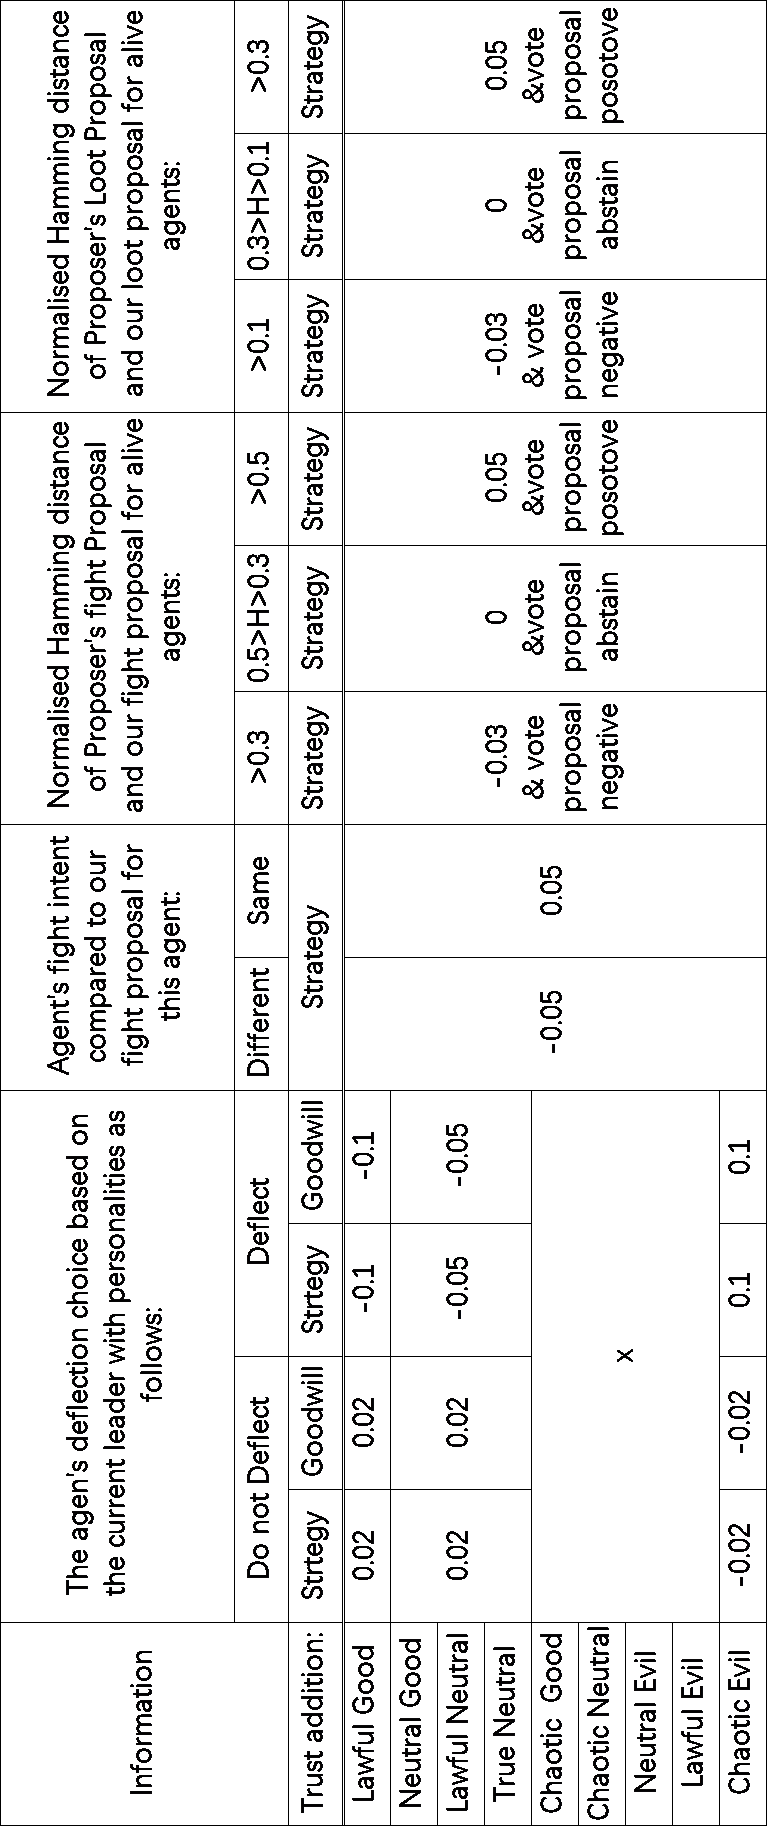
\includegraphics[scale=1]{008_team_5_agent_design/images/Information2Trusts.png}

\begin{figure}[htb]
    \caption{Details of updating trusts regarding different information that can be collected.}
    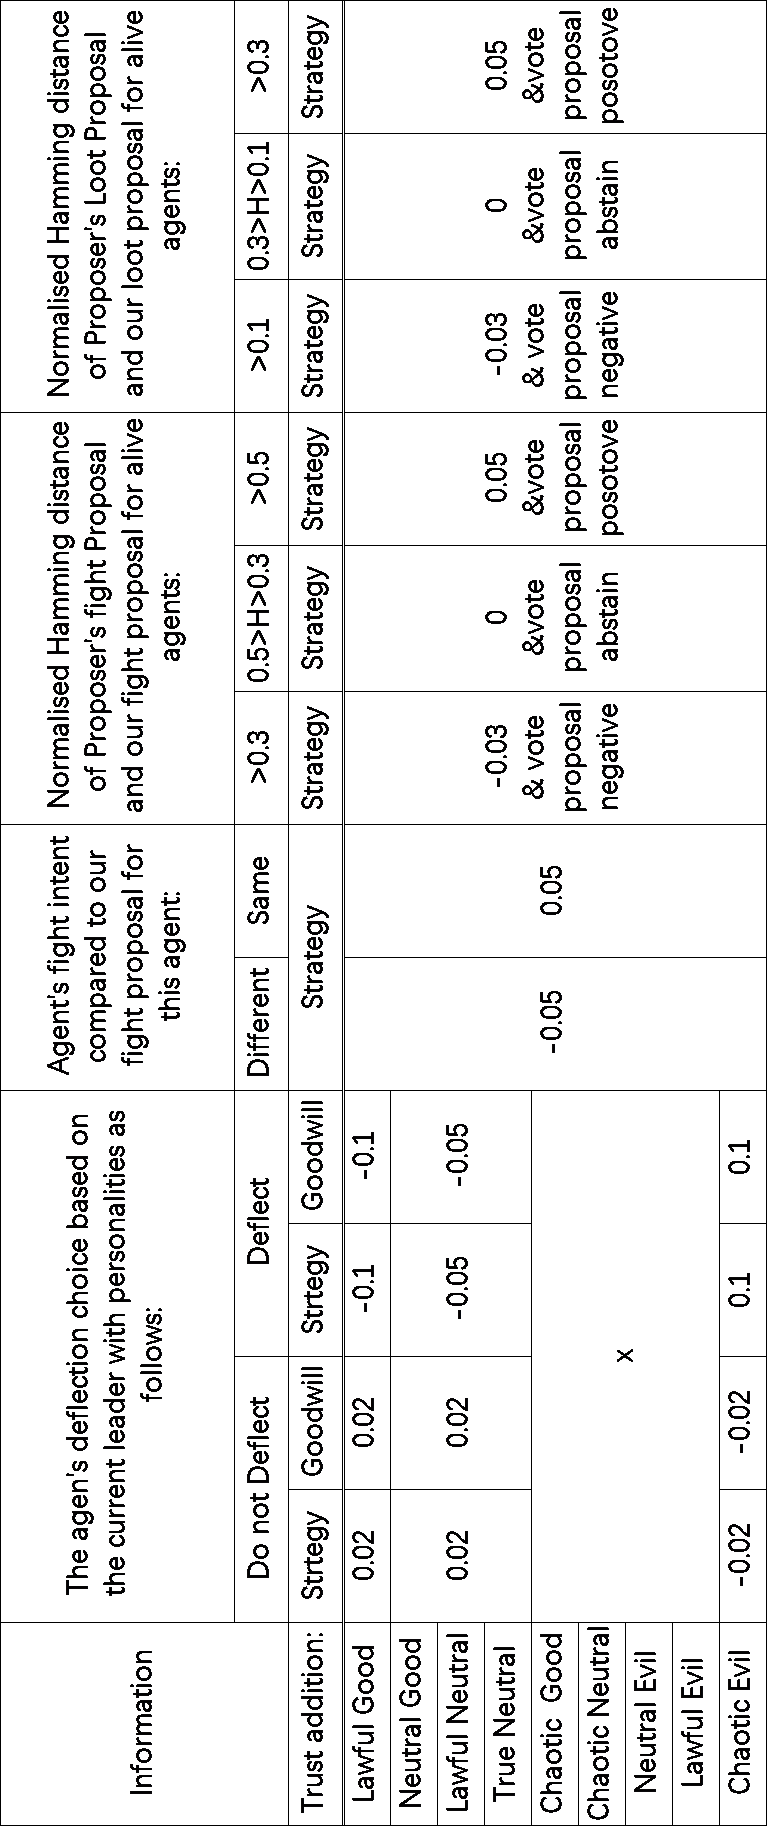
\includegraphics[width=0.60\textwidth]{008_team_5_agent_design/images/Information2Trusts.png}
    \label{fig:Information2Trusts}
\end{figure}
\clearpage

\begin{figure}[htb]
    \centering
    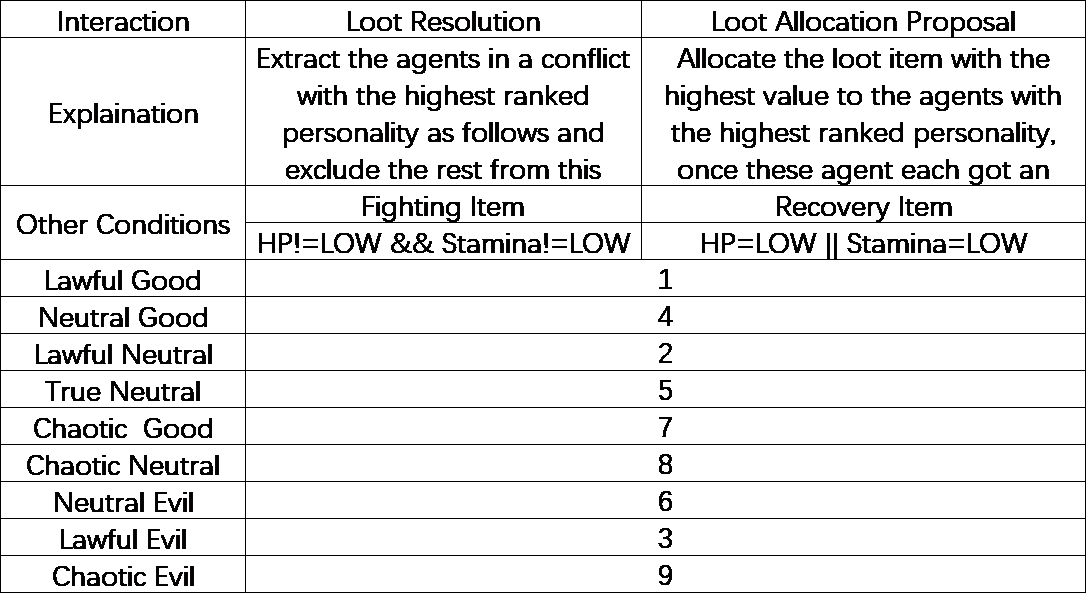
\includegraphics[scale=0.5]{008_team_5_agent_design/images/Interaction.png}
    \caption{Other agents' personality impact on our agent's interaction behaviour}
    \label{fig:my_label}
\end{figure}


\section{Election}

\section{Leadership Logic}
\subsection{Fight Logic}
\noindent As mentioned in leadership personality, our agent aims to maximize utility by prioritizing taking the least total damage and deaths when making fight decisions.There are 2 fighting conditions where the level can be passed without taking any damage or deaths. The leader fight algorithm will first check for the following two criterions: 

\begin{enumerate}
\item  $\sum{Agent~Attack>Monster~Resilience}$
\

\noindent If the sum of Agent's attack values is greater than monster resilience, we are capable of defeating the monster in one fight round without giving it the opportunity to deal damage.

\item  $\sum{Agent~Shield>Monster~Attack}$


\noindent If the sum of Agent's shield values is greater than monster attack, we will receive no incoming damage.
\end{enumerate}
\noindent If either criterion is met, the fight decision is determined by minimizing stamina consumption:

\begin{enumerate}
\item  Agents are ranked according to their attack values. The agent's attack values are summed iteratively starting with the agent with the highest attack value, this is compared against monster resilience for each iteration. Once summed attack is greater than monster resilience, the agent's included in the sum are chosen to attack and all other agents will cower. This ensures we will not deal excessive damage to the monster and waste stamina points that could be utilized in later levels. As agents won't receive damage, their health points are not taken into consideration, meaning low health point agents can still fight.

\noindent 

\item  Agents are ranked according to their shield values. The agent's shield values are summed iteratively starting with the agent with the highest shield value, this is compared against monster attack for each iteration. Once summed shield is greater than monster attack, the agent's included in the sum are chosen to defend and all other agents will attack in order to defeat the monster with least number of fighting rounds.
\end{enumerate}

\noindent 

\noindent If neither criterion can be met, the algorithm will determine whether to prioritize taking the least damage or least deaths by comparing the percentage of surviving agents to a threshold determined by the current level. If percentage of surviving agents is greater than the threshold, the algorithm with prioritize taking the least amount of damage and vice versa. The threshold is set at 90\% for the first 10 levels, then linearly decreases to 60\% (criteria to win game) at the final level.

\noindent 

\noindent Once priority is decided, all agents are ranked with respect to health points from high to low. A comparison of the agent's attack and shield value will determine their fight decision, this is done iteratively starting with the agent ranked first. We define total attack as the sum of agent attack values with an attack fight decision, and total shield as the sum of agent shield values with a defend fight decision. Agent's that attack will have 0 shield and agents defending has 0 attack. The first iteration will include only the first agent, such that if the fight decision is attack the total attack would equal to the agent's attack value and shield would be 0. The second iteration will include the first and second ranked agents, this is shown with the figure below:
\begin{figure}[htb]
    \centering
    \includegraphics[width=1\textwidth]{008_team_5_agent_design/images/Rank-all-Agents-by-hp.png}
    \caption{Agents are ranked based on thier health points}
    \label{rankagents}
\end{figure}


\noindent Using number of fighting agents, total attack and total shield, the algorithm will determine the estimated damage taken by all agents and expected number of agent deaths. Dividing monster resilience by total attack, we can solve for the number of fighting rounds required to defeat the monster. 
\[Fighting\ Rounds\ to\ Kill\ Monster\approx \frac{Monster\ Resilience}{Total\ Attack}=R\] 
Using monster attack, total shield, and number of fighting agents we can determine the damage to individual agents per round as:
\[Damage\ to\ Individual\ Agent\ Per\ Round=\frac{Monster\ Attack\mathrm{-}Total\ Shield}{Number\ of\ Fighting\ Agents\ (N)}\ =D_R\] 
Therefor total damage received by agents can be calculated by:
\[Total\ damage\ received\ by\ agents=\ D_R\ \times \ N\ \times R=\ D_T\] 
Using $D_R$ we can obtain the damage received by an individual agent to pass the level:
\[Damage\ received\ by\ agent\ to\ pass\ level=\ D_R\times \ R\ =D_P\] 
And agent deaths are determined by the number of agents with health points lower than $D_P$

\noindent To ensure total attack and total shield values are not skewed, each agent's attack values were scaled 5 times with factors between 0.5 and 2 when determining their fight decision. Continuing our figure example, we can see below in figure how individual agent fight decisions can change.
\begin{figure}[htb]
    \centering
    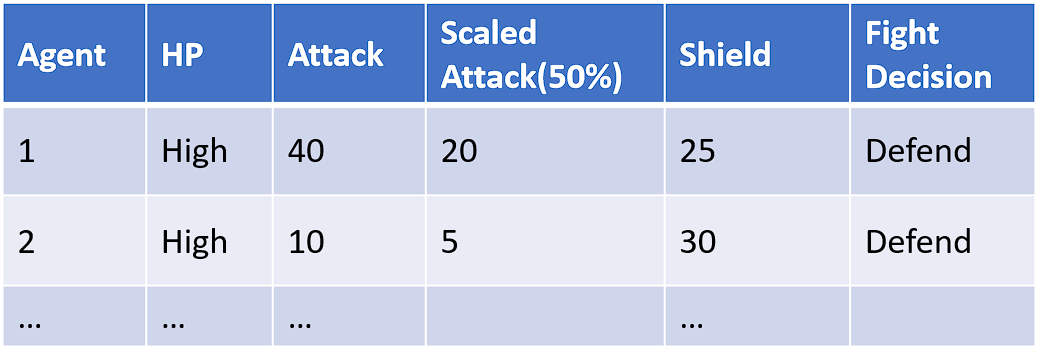
\includegraphics[width=1\textwidth]{008_team_5_agent_design/images/scaled-attack.PNG}
    \caption{Agent attack values are scaled by 50\%}
    \label{scaledattack}
\end{figure}

\noindent The scaling factors will give a more comprehensive view for different agent fight decision combinations, hence increasing our likelihood of finding a fight solution that is truly optimal. If all agents are alive, there could be up to 100 iterations for each of the 5 scaled attacks. But by performing each iteration in parallel, we can reduce the execution time and ensure time constraints are met.

\noindent If the number of fighting agents exceeds the calculated number of deaths for the iteration, the level is passed. From the iterations that meet this criterion, the one which optimizes for least damage or least deaths are chosen with regards to our predetermined priority. The algorithm will finally return a fight decision map reflecting our best fight solution for the current level. 



\subsection{Loot Allocation}
\subsection{Manifesto}



\section{Fight Logic}
The fighting stage could be viewed as a Markov decision process, where from the current state, an agent could have certain probability to transit into another state (new or same), by performing one of the three fighting actions, Attack / Defend / Cower.

The state space $S$ is designed based on level of health, stamina, attack, defence of an agent. 

\noindent

\begin{table}[!ht]
\begin{tabular}{|l|l|l|l|}
\hline
\begin{tabular}[c]{@{}l@{}}Health \\ (to init health)\end{tabular}                      & \begin{tabular}[c]{@{}l@{}}Stamina \\ (to init stamina)\end{tabular}                    & \begin{tabular}[c]{@{}l@{}}Attack \\ (to observable agents)\end{tabular}          & \begin{tabular}[c]{@{}l@{}}Defence \\ (to observable agents)\end{tabular}         \\ \hline
\textit{\begin{tabular}[c]{@{}l@{}}Low\\ hp \textless 30\%\end{tabular}}                & \textit{\begin{tabular}[c]{@{}l@{}}Low\\ ap \textless 30\%\end{tabular}}                & \textit{\begin{tabular}[c]{@{}l@{}}Weakee\\ AT \textless 25\%\end{tabular}}       & \textit{\begin{tabular}[c]{@{}l@{}}Weakee\\ SH \textless 25\%\end{tabular}}       \\ \hline
\textit{\begin{tabular}[c]{@{}l@{}}Mid\\ 30\% \textless hp \textless 60\%\end{tabular}} & \textit{\begin{tabular}[c]{@{}l@{}}Mid\\ 30\% \textless ap \textless 60\%\end{tabular}} & \begin{tabular}[c]{@{}l@{}}Ordina\\ 25\% \textless AT \textless 75\%\end{tabular} & \begin{tabular}[c]{@{}l@{}}Ordina\\ 25\% \textless SH \textless 75\%\end{tabular} \\ \hline
\begin{tabular}[c]{@{}l@{}}High\\ 60\% \textless hp\end{tabular}                        & \begin{tabular}[c]{@{}l@{}}High\\ 60\% \textless ap\end{tabular}                        & \begin{tabular}[c]{@{}l@{}}Master\\ 75\% \textless AT\end{tabular}                & \begin{tabular}[c]{@{}l@{}}Master\\ 75\% \textless SH\end{tabular}                \\ \hline
\end{tabular}
\end{table}

So in total there's 81 different states. The attack / defence intervals are separated assuming normal distribution, so extremes are less common and are valuable to treat differently.

In terms of decision, our agent utilise the Q learning algorithm, where each agent keeps a map of Q values and the action taken from last state, these Q values are updated throughout the game according to feedback (reward) on the action taken at certain state.

Updates rule:

$Q(S,A) \leftarrow Q(S,A) + \alpha(R(S,A) + \gamma \max\limits_{A^+} Q(S^+,A^+) - Q(S,A))$

The Q value for a state-action association pair represents how much an agent favour a specific action at a given state. So the strategy for an agent is to follow the highest Q value most of time, but allow some random deviation from that to explore the unknowns.



\section{Trading Logic}



\section{Experiment}

\subsection{Leader Fight Logic}
The leader fight logic’s execution time was tested to ensure it is within the time limit of 0.5 seconds. 

\noindent

\begin{figure}[htb]
    \centering
    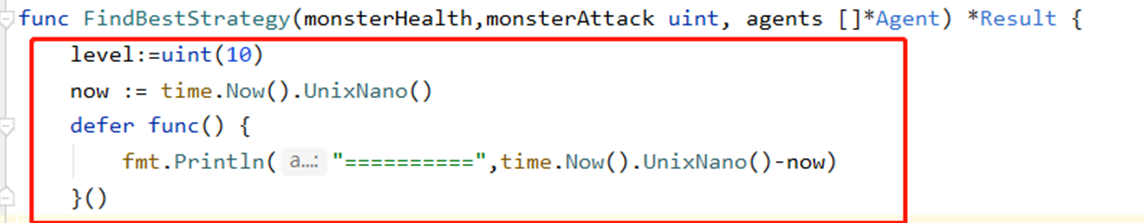
\includegraphics[width=0.7\textwidth]{008_team_5_agent_design/images/10.png}
    \caption{Measuring execution time}
    \label{testingexecutiontime}
\end{figure}

\noindent   

\begin{figure}[!ht]
    \centering
    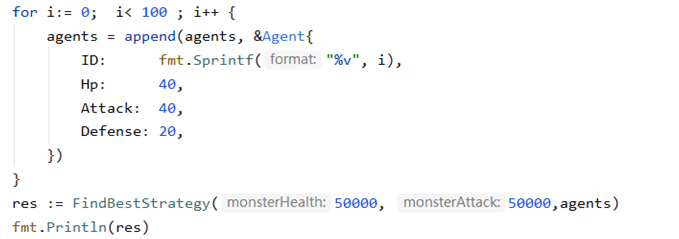
\includegraphics[width=0.7\textwidth]{008_team_5_agent_design/images/11.png}
    \caption{Initialising Agent and Monster}
    \label{initialisingagentandmonster}
\end{figure}

\noindent

\noindent Some results are shown below, execution time is labelled with consumer in units of nano seconds.

\noindent

\begin{figure}[!ht]
    \centering
    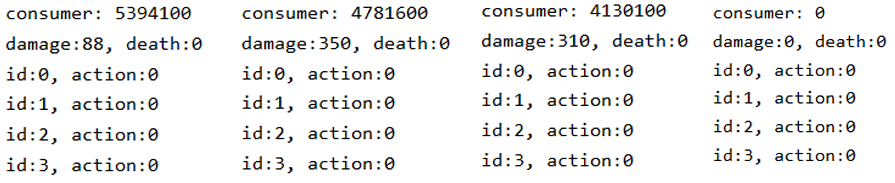
\includegraphics[width=0.7\textwidth]{008_team_5_agent_design/images/12.png}
    \caption{Execution time test results}
    \label{executiontimetestresults}
\end{figure}

\noindent

\noindent All trials had execution time under 0.01 seconds and well below the time limit.

